% Focused 3D scale-mode regression, derived from PGFPlots scaling semantics.
\documentclass[tikz,border=2pt]{standalone}
\usepackage{pgfplots}
\pgfplotsset{compat=newest}
\begin{document}
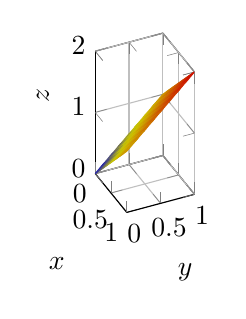
\begin{tikzpicture}
  \begin{axis}[
    width=6cm,
    height=3cm,
    scale only axis,
    scale mode=scale uniformly,
    scale uniformly strategy=units only,
    view={65}{35},
    xmin=0, xmax=1,
    ymin=0, ymax=1,
    zmin=0, zmax=2,
    grid=major,
    xlabel={$x$}, ylabel={$y$}, zlabel={$z$}
  ]
    \addplot3[surf,domain=0:1,y domain=0:1,samples=9] {x + y};
  \end{axis}
\end{tikzpicture}
\end{document}
